%% This is file `DEMO-TUDaExercise.tex' version 2.10 (2020/04/26),
%% it is part of
%% TUDa-CI -- Corporate Design for TU Darmstadt
%% ----------------------------------------------------------------------------
%%
%%  Copyright (C) 2018--2020 by Marei Peischl <marei@peitex.de>
%%
%% ============================================================================
%% This work may be distributed and/or modified under the
%% conditions of the LaTeX Project Public License, either version 1.3c
%% of this license or (at your option) any later version.
%% The latest version of this license is in
%% http://www.latex-project.org/lppl.txt
%% and version 1.3c or later is part of all distributions of LaTeX
%% version 2008/05/04 or later.
%%
%% This work has the LPPL maintenance status `maintained'.
%%
%% The Current Maintainers of this work are
%%   Marei Peischl <tuda-ci@peitex.de>
%%   Markus Lazanowski <latex@ce.tu-darmstadt.de>
%%
%% The development respository can be found at
%% https://github.com/tudace/tuda_latex_templates
%% Please use the issue tracker for feedback!
%%
%% ============================================================================
%%
% !TeX program = lualatex
%%

%=========================================================

% Here you can choose to compile with or without solutions.
% However, this definition is ignored if you use any
% command from the `Makefile`.
%\providecommand{\withSol}{\iftrue}

%=========================================================


\documentclass[
	colorback=false,
	solution=true,
	]{tudaexercise}

\usepackage[english, main=english]{babel}
\usepackage[babel]{csquotes}
\usepackage{amsmath}
\usepackage{booktabs}
%~~~~~~~~~~~~~~~~~~~~~~~~~~~~~~~~~~~~~~~~~~~~~~~~~~~~~~~~~
% Zusätliche Pakete
\usepackage{comment}
\newcommand{\urlc}[1]{\color{cyan}\url{#1}\color{black}}
\newcommand{\hrefc}[2]{\color{cyan}\href{#1}{#2}\color{black}}
\newcommand{\prog}[1]{\textit{#1}}
\newcommand{\concept}[1]{\textbf{#1}}
\newcommand{\codesym}{\textbf{\texttt{</>}}}
\usepackage{cite}
\usepackage{dirtree}
\usepackage{amssymb}
\usepackage{tikz}
\usepackage{textcomp}
\usepackage{url}
\usepackage[newenum]{paralist}
\usepackage{bbding}
\usepackage{float}
\usepackage{listings}

% The (in)famous algorithm package
\usepackage[vlined,linesnumbered]{algorithm2e}
\SetArgSty{textnormal}
\SetCommentSty{textit}
\usepackage{wrapfig}
\usepackage{nicefrac}
\usepackage{multicol}
\usepackage{multirow}

% Write `B+-tree' consistently throughout the lecture
\newcommand{\Btree}{B\raisebox{.4em}{\textsmaller{+}}-tree}
\newcommand{\Btrees}{B\raisebox{.4em}{\textsmaller{+}}-trees}
\newcommand{\BTree}{B\raisebox{.4em}{\textsmaller{+}}-Tree}
\newcommand{\BTrees}{B\raisebox{.4em}{\textsmaller{+}}-Trees}
\newcommand{\BBaum}{B\raisebox{.4em}{\textsmaller{+}}-Baum}
\newcommand{\BBaums}{B\raisebox{.4em}{\textsmaller{+}}-Baums}
\newcommand{\BBaeume}{B\raisebox{.4em}{\textsmaller{+}}-Bäume}
\newcommand{\R}[0]{\mathds{R}} % real numbers
%~~~~~~~~~~~~~~~~~~~~~~~~~~~~~~~~~~~~~~~~~~~~~~~~~~~~~~~~~

%\usepackage{biblatex}
%=========================================================

\def\homework{3}
\def\homeworkVer{1}
\def\homeworkSolVer{1}
%=========================================================

%Formatierungen für Beispiele in diesem Dokument. Im Allgemeinen nicht notwendig!
\let\file\texttt
\let\code\texttt
\let\pck\textsf
\let\cls\textsf
\let\tbs\textbackslash

\ConfigureHeadline{
	headline={title-name-id}
}

%compatbilitx
\let\unit\relax

\begin{document}

\title{Statistical Machine Learning Homework 3}
\author{Patrick Nowak\\Rinor Cakaj}
\term{Sommersemester 2020}
\date{\today}
\sheetnumber{\homework}
\setcounter{section}{\homework}

\maketitle

\begin{task}[]{PCA}
 We use the data-set \text{iris.txt}. Each row in it has 4 Attributes and a label(classification).
 \begin{subtask}
 	We normalize the data, s.t. every Attribute has mean zero and variance 1. Therefore, for every column, we compute the sample mean and subtract it. Then, we devide by the standard deviation. Of course, this is only done for the columns containing attributes.
 	\begin{figure}[H]
 		\begin{lstlisting}[language=python]
	#3a
	n = len(iris)
	pre_iris = iris[:,0:4]
	pred = iris[:,4]
	mean = pre_iris.mean(0)
	step1 = pre_iris - mean
	standard_deviation=np.std(pre_iris, axis=0)
	normalized_data = np.multiply(step1, 1/standard_deviation).T   
 		\end{lstlisting}
 	\end{figure}
	\text{"normalized\_data"} does now contain one row per attribute, each row having mean zero and variance one.
\end{subtask}
\begin{subtask}
	We apply PCA on the normalized dataset. We plot a bar graph where the \text{i-th} bar shows how much of the original variance we already captured using the biggest \text{i} components.
\begin{lstlisting}[language=python]
def PCA(normalized_data):
	cov = np.cov(normalized_data)
	eigenvalues, eigenvectors = np.linalg.eig(cov)
	
	summe = np.sum(eigenvalues)
	eigenvalues_prop = eigenvalues/summe
	
	ind = [1,2,3,4]
	kum = np.zeros(4)
	kum[0] = eigenvalues_prop[0]
	for i in range(1,4):
		kum[i]=kum[i-1] + eigenvalues_prop[i]  
	kum=kum*100
	plt.bar(ind, kum)
	rounded=np.round(kum,2)
	for idx,y in enumerate(rounded):
	plt.text(ind[idx]-0.2,y+1,str(y)+"%")
	plt.show()    
	return eigenvalues, eigenvectors
\end{lstlisting}
Calling the function produces the following plot:
\begin{figure}[H]
	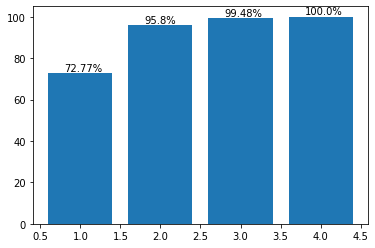
\includegraphics[]{bar}
\end{figure}
We see that for two components we explained already more than 95\% of the variance.
\end{subtask}
\begin{subtask}
	We do the PCA for the two biggest components. We wrote the following function:
\begin{lstlisting}[language=python]
	def threec(eigenvalues, eigenvectors, normalized_data, pred):
		B = eigenvectors[:,0:2]
		normalized_data_p = np.matmul(B.T, normalized_data)
		normalized_data_p = np.vstack((normalized_data_p, pred))
		colors = ['red','green','blue']
		plt.scatter(normalized_data_p[0], normalized_data_p[1], 
			c=normalized_data_p[2], cmap=matplotlib.colors.ListedColormap(colors))
		return
\end{lstlisting}
The first input arguments are clear, in the last argument we give the real data values from iris.txt just without the classification column. We then used the first two eigenvalues for projection on the $R^2$. Calling it, we get
\begin{figure}[H]
		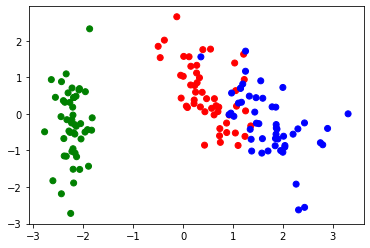
\includegraphics[]{2dprojectionPCA}
\end{figure}
where we used different colors for different classes(red=Setosa,green=Versicolour,blue=Virginica). We observe, that the green dots are well separated from the rest. Therefore we can argue, that Versicolour is pretty unique compared to the other two. For the red and blue dots it can be harsh to find a good decision boundary around x=1 we got both blue and red samples. The Setosa and the Virginica data seem to have more in common. Though, if we go away from the boundary, we could use the points to get - at least on the given training data - a very clear classification.
\end{subtask}
\begin{subtask}
We perform the PCA for n=1,2,3,4 components. Then we take the computed points from $R^{n}$ and embed them in $R^4$ to calculate an error distance. Doing this, we need to consider the normalization we have on our \text{normalized\_data}, which was, for real dataset X with mean $\bar{x}$ and variance $\text{std}^2$ 
\begin{align*}
normalized\_data=\frac{X-\bar{x}}{std}\\
\end{align*}
Following the idea of slide 27 in lecture 10, we get
\begin{align*}
a^n&=B^T\cdot\left( X-\bar{x}\right) \\&= B^T\cdot\left( normalized\_data \cdot std\right) \\
\\
\tilde{x}^n&=\bar{x}+B\cdot a^n
\end{align*}
where B is the matrix of the first n eigenvalues. We implemented this backtransformation in the comp\_set function.
\begin{lstlisting}[language=python]
def comp_set(n, eigenvectors, normalized_data, mean, var):
	B = eigenvectors[:,0:n+1]
	normalized_data_p = np.matmul(B.T, normalized_data) 
	reconstruction = np.matmul(B, normalized_data_p)
	rec=np.multiply(reconstruction.T,var)
	rec=rec+mean
	return rec
\end{lstlisting}
Now, we can compare the backtransformed data to the original uncompressed data via normalized mean squared error.
\begin{lstlisting}[language=python]
def rmse(x):
	return np.sqrt(np.mean(x**2))

def threed(eigenvalues, eigenvectors, normalized_data, pre_iris, mean, var):
	lsg=np.zeros([4,4])
	for comp in range(4):
		re = comp_set(comp, eigenvectors, normalized_data, mean, var)
		diff = re - pre_iris
	for feature in range(4):
		lsg[comp,feature]=rmse(diff[:,feature])/
			(np.sum(pre_iris[:,feature]/len(pre_iris)))
	print("lsg:", lsg)
	return 
\end{lstlisting}
Calling the threed function gives us the following solution:
\begin{table}[H]
	\begin{tabular}{lllll}
		& x\_1    & x\_2     & x\_3    & x\_4     \\
		n=1 & 6.406\% & 12.641\% & 6.021\% & 16.642\% \\
		n=2 & 3.945\% & 1.339\%  & 5.946\% & 16.158\% \\
		n=3 & 0.531\% & 0.252\%  & 5.381\% & 4.769\%  \\
		n=4 & 0       & 0        & 0       & 0       
	\end{tabular}
\end{table}
\end{subtask}
\end{task}



%\bibliography{library}{}
%\bibliographystyle{plain}

\end{document}
